\documentclass[aps,pra,reprint,superscriptaddress,longbibliography]{revtex4-2}
\usepackage[UTF8,scheme=plain,fontset=fandol]{ctex}
\usepackage{amsmath,amssymb,amsthm,mathtools}
\usepackage{graphicx}
\usepackage[colorlinks=true,linkcolor=blue,citecolor=blue,urlcolor=blue]{hyperref}
\newtheorem{theorem}{定理}
\newtheorem{lemma}[theorem]{引理}
\newtheorem{proposition}[theorem]{命题}
\newtheorem{corollary}[theorem]{推论}
\theoremstyle{remark}
\newtheorem{remark}[theorem]{注}
\renewcommand{\proofname}{证明}
\renewcommand{\appendixname}{附录}
\renewcommand{\figurename}{FIG.}
\renewcommand{\tablename}{TABLE}
\DeclareMathOperator{\tr}{tr}
\DeclareMathOperator{\Var}{Var}
\DeclareMathOperator{\Cov}{Cov}
\DeclareMathOperator{\diag}{diag}
\newcommand{\E}{\mathbb E}
\newcommand{\R}{\mathbb R}
\newcommand{\C}{\mathbb C}
\newcommand{\id}{I}
\newcommand{\abs}[1]{\lvert#1\rvert}
\newcommand{\norm}[1]{\lVert#1\rVert}
\newcommand{\ket}[1]{\lvert#1\rangle}
\newcommand{\bra}[1]{\langle#1\rvert}
\newcommand{\ip}[1]{\langle#1\rangle}
\newcommand{\nh}{\mathrm{NH}}
\newcommand{\g}{\mathrm G}

\newcommand{\scalingcaption}{%
Finite-copy behavior in two-parameter qubit estimation at the maximally
mixed state. The Gaussian positive operator-valued measure (POVM) uses
$\epsilon_j=1/\log(e+j+1/2)$.
(a) Average planar variance divided by spin: the Gaussian value
$W_j^{\g}/j$ (circles), the all-POVM lower bound $L_j/j$ (squares),
and the spin-coherent value $2/3$ (dotted line).
The dashed horizontal line marks the optimal limit $1/2$.
(b) Normalized risk correction $\sqrt{N}(C-2)$ for
$C=C_N^{\g}$ (circles) and the Nagaoka--Hayashi (NH) lower bound
$C=C_N^{\nh}$ (squares), with $C$ equal to $N$ times the total mean squared error.
The dashed horizontal line marks their common limit $\sqrt{8/\pi}$.
Both horizontal axes are logarithmic; lines joining numerical points
guide the eye. Points are obtained by numerical quadrature, while the
limiting values follow analytically. The Gaussian scheme attains the
optimal first correction and is not asserted to be optimal at each finite $N$.}


\begin{document}
\title{双参数量子比特估计中的首个有限拷贝修正}
\author{Tingyu Zhang}
\email{23300190021@m.fudan.edu.cn}
\affiliation{复旦大学物理系，上海，中国}
\author{Yan Cen}
\email[通讯作者：]{cenyan@fudan.edu.cn}
\affiliation{复旦大学物理系，上海，中国}

\date[]{}
\begin{abstract}
对有限个量子态拷贝进行联合测量，必须权衡不相容自旋分量的信息。
精度趋于无限拷贝极限的过程受到测量完备性约束。
本文求得最大混合态处双参数量子比特估计的可达局部无偏风险的首个有限拷贝修正。
对 $N$ 个拷贝的联合测量进行优化，总均方误差乘以 $N$ 后的最优值为
$2+\sqrt{8/\pi}\,N^{-1/2}+o(N^{-1/2})$。
核心结果是：在自旋 $j$ 的最大混合态 $I/(2j+1)$ 处，两个横向自旋方差的共同凸屋顶等于 $j/2+o(j)$。
我们构造宽度随位置变化的高斯列，使每一列的布居积分严格等于一，
再以有限相位平均对每个有限自旋构成完备的正算子值测度。
一致的能量估计与匹配的平方和下界共同确定最优修正。
一个显式宽度序列及相应的得分估计量达到这一修正，同时对每个有限 $N$ 保持严格局部无偏。
因此，对 $N\geq10$ 存在的严格有限拷贝 Nagaoka--Hayashi 间隙，
对归一化风险仅贡献 $o(N^{-1/2})$。
\end{abstract}

\maketitle

\section{引言}\label{sec:introduction}

多参数量子估计的有限拷贝精度，取决于如何在一次测量中获取不相容观测量的信息。
即使无限拷贝极限已知，构造达到其首阶修正的完备测量仍是一个独立问题。
本文研究最大混合态处量子比特两个笛卡尔分量的这一问题。

锥规划刻画了可达局部风险，并允许重建完备测量\cite{HayashiOuyang2023}。
Schur--Weyl 约化进一步简化了有限拷贝优化\cite{ZhangHayashi2026}。
这些方法提供了有限维框架，但固定 $N$ 下测量网格的收敛，
不能确定最优风险趋于无限拷贝极限的速率。
本文既要确定随拷贝数增长的修正，也要给出达到该修正的显式正算子值测度（POVM）族。

平面自旋压缩与低方差自旋态的高斯描述提供了局部构造所需的工具\cite{He2011,Dammeier2015}。
特别地，文献\cite[定理~4]{Dammeier2015}中的固定压缩渐近结果经旋转与优化后，
在固定非零纬度 $x$ 处给出局部代价 $j|x|$，其形式平均为
$j\int_{-1}^1|x|\,dx/2=j/2$。
要实现这一平均值，还需得到 $I/d$ 的精确分解：分别选取的低方差态未必具有所需的平均布居。
我们先将每一高斯列归一化，再进行相位平均，从而严格满足这一约束，
并控制整个自旋扇区内的平均方差。

这一构造结合适用于全部 POVM 的下界，给出最优归一化风险
$C_N=2+\sqrt{8/\pi}\,N^{-1/2}+o(N^{-1/2})$。
显式测量族的每个有限成员均严格完备，并配有严格局部无偏的估计量。
同一分析表明，对 $N\geq10$ 存在的严格有限拷贝 Nagaoka--Hayashi（NH）间隙，
在 $N^{-1/2}$ 尺度上是次阶的。证明将精确布居归一化、一致能量估计与 Schur 扇区平均连接起来。

\section{模型与可达精度}\label{sec:model}\label{sec:reduction}

考虑满秩的局部量子比特模型
\begin{equation}
 \rho_{x,y}=\frac12(I+x\sigma_x+y\sigma_y),\qquad x^2+y^2<1,
 \label{eq:model}
\end{equation}
在 $(x,y)=(0,0)$ 处的估计问题，其中 $\sigma_x$ 与 $\sigma_y$ 为 Pauli 矩阵。
参数为 Bloch 向量的笛卡尔分量。
对每个正整数 $N$，在 $\rho_{x,y}^{\otimes N}$ 上施加一次任意联合 POVM，
其测量结果可以离散或连续。要求估计量 $\widehat\theta=(\widehat x,\widehat y)$ 满足
\begin{equation}
 \E_0\widehat\theta_a=0,\qquad
 \left.\partial_{\theta_b}\E_\theta\widehat\theta_a\right|_0
 =\delta_{ab},\qquad \theta=(x,y),
 \label{eq:unbiased}
\end{equation}
并定义
\begin{equation}
 C_N=N\inf_{M,\widehat\theta}
 \E_0(\widehat x^2+\widehat y^2).
 \label{eq:risk}
\end{equation}
测量与估计量均可依赖于参考点。辅助系统、经典随机化、测量结果数目及效应算子的秩均不受限制。

取 $\hbar=1$，记 $J_x,J_y,J_z$ 为自旋 $j$ 的角动量算符，$d=2j+1$。
相关的共同方差凸屋顶为
\begin{equation}
 V_j=\min_{\sum_a p_a\ket{\psi_a}\bra{\psi_a}=I/d}
 \sum_a p_a\bigl(\Var_{\psi_a}J_x+\Var_{\psi_a}J_y\bigr).
 \label{eq:roof}
\end{equation}
其中 $p_a$ 为概率，$\psi_a$ 为归一化纯态。两个方差使用同一个分解。
这类共同凸屋顶属于基于纯态分解的不确定性关系的一般框架\cite{TothFrowis2022}。

令 $\mathcal J_N=\{j_{\min},j_{\min}+1,\ldots,N/2\}$，其中偶数 $N$ 对应
$j_{\min}=0$，奇数 $N$ 对应 $j_{\min}=1/2$。Schur 分解及其在参考点处的概率为
\begin{equation}
\begin{aligned}
(\C^2)^{\otimes N}
 &=\bigoplus_{j\in\mathcal J_N}\mathcal H_j\otimes\C^{\nu_j},\\
\nu_j&=\binom N{N/2-j}-\binom N{N/2-j-1},\\
P_{N,j}&=\frac{(2j+1)\nu_j}{2^N}.
\end{aligned}
\label{eq:schur}
\end{equation}
下标超出范围时，二项式系数取零。给定 $j$，参考态及其两个切向算符为
\begin{equation}
 Q_j=\frac{I}{d},\qquad \dot Q_{j,x}=\frac{2J_x}{d},\qquad
 \dot Q_{j,y}=\frac{2J_y}{d}.
 \label{eq:tangents}
\end{equation}
概率 $P_{N,j}$ 关于两个参数的一阶导数均为零。记 $\E_N$ 为概率 $P_{N,j}$ 下的期望。

\begin{lemma}\label{lem:reduction}

若 $T_j$ 是自旋 $j$ 模型 \eqref{eq:tangents} 中经典 Fisher 信息矩阵迹的最大值，则
\begin{equation}
\begin{aligned}
T_N&=\sum_jP_{N,j}T_j,\qquad C_N=\frac{4N}{T_N},\\
T_j&=\frac83j(j+1)-4V_j.
\end{aligned}
\label{eq:reductions}
\end{equation}
这些恒等式对全部 POVM 成立，无需额外的样本量极限。

\end{lemma}

证明见附录~\ref{app:reduction}，其中包括任意复效应算子及连续测量结果的处理。
最大值可以达到，因此该优化对每个有限 $N$ 都定义了可达的局部风险。

\section{最优有限拷贝修正}\label{sec:result}

\begin{theorem}\label{thm:main}

当 $j$ 沿整数或半整数自旋趋于无穷时，
\begin{equation}
 V_j=\frac j2+o(j).
 \label{eq:roof-asymptotic}
\end{equation}
对模型 \eqref{eq:model}，在所有联合 POVM 及所有满足 \eqref{eq:unbiased} 的估计量上优化，有
\begin{equation}
 \boxed{\displaystyle
 C_N=2+\sqrt{\frac8\pi}\,N^{-1/2}+o(N^{-1/2}).}
 \label{eq:main}
\end{equation}
第~\ref{sec:gaussian}~节的高斯列测量取
\begin{equation}
 \epsilon_j=\frac1{\log(e+j+1/2)},\qquad j>0,
 \label{eq:epsilon}
\end{equation}
并配合式 \eqref{eq:estimator} 的估计量，对每个正整数 $N$ 均有良好定义，
测量严格完备，估计量严格局部无偏。其风险具有相同的展开式 \eqref{eq:main}。

\end{theorem}

式 \eqref{eq:main} 的系数由各自旋扇区内恒等算子完备分解的代价决定。
附录~\ref{sec:lower} 给出适用于所有 POVM 的平方和证书，其下界为 $L_j=j/2+o(j)$。
附录~\ref{sec:energy-proof} 证明严格完备的高斯测量族具有平均方差 $W_j^{\g}=j/2+o(j)$。
因此，$L_j\leq V_j\leq W_j^{\g}$ 确定了自旋渐近行为。

Schur 平均自旋满足 $\mathbb E_N j/\sqrt N\to\sqrt{2/\pi}$。
对任意固定的自旋序列 $r_j=o(j)$，附录~\ref{sec:averaging} 将有限个小自旋项与大自旋项直接分开，
证明 $\mathbb E_N r_j=o(\sqrt N)$。因此，关于 $j$ 首阶线性的方差代价，
在平均后成为 $\sqrt N$ 阶的 Fisher 信息损失。
式 \eqref{eq:reductions} 再将这一损失转化为归一化风险的 $N^{-1/2}$ 修正。
特别地，证明涵盖 $N$ 的两种奇偶性，并包含全部小自旋扇区。

\section{完备测量}\label{sec:gaussian}

固定 $j>0$，令 $J=j+1/2$。先取正函数 $b\in C^2([-1,1])$，并定义
\begin{equation}
\begin{aligned}
a(x)&=(1-x^2)b(x),\qquad S(s)=Ja(s/J),\\
v_s(t)&=(2\pi S(s))^{-1/4}
 \exp\!\left[-\frac{(t-s)^2}{4S(s)}\right],\\
&\hspace{35mm}|s|\leq j.
\end{aligned}
\label{eq:columns}
\end{equation}
取 $m=-j,\ldots,j$ 的离散列 $v_m(t)$。令 $c_m=\sqrt{(j-m)(j+m+1)}$，并记
\begin{equation}
\begin{aligned}
s_j(t)&=\sum_m v_m(t)^2,\\
h_j(t)&=\sum_{m=-j}^{j-1}c_mv_m(t)v_{m+1}(t).
\end{aligned}
\label{eq:sh}
\end{equation}
对整数 $L\geq\max(d,3)$，令 $\phi_\ell=2\pi\ell/L$，$\ell=0,\ldots,L-1$，并定义 POVM 密度
\begin{equation}
\begin{aligned}
E_j(dt,\ell)&=\frac1L\ket{v_{t,\ell}}\bra{v_{t,\ell}}\,dt,\\
\ket{v_{t,\ell}}&=\sum_m v_m(t)e^{-im\phi_\ell}\ket m.
\end{aligned}
\label{eq:gaussian-povm}
\end{equation}
由于 $|m|\leq J-1/2$，每个 $S(m)>0$。
各效应算子均为正，且 $\int_\R v_m(t)^2\,dt=1$。
相位平均严格消去全部非对角元，因此
\begin{equation}
 \sum_{\ell=0}^{L-1}\int_\R E_j(dt,\ell)=I.
 \label{eq:complete}
\end{equation}
因此，列归一化固定恒等算子的对角元，相位平均消去非对角元。
这一完备性关系在整个实数结果空间上成立。相应的 $I/d$ 分解具有密度 $s_j(t)/(dL)$ 和归一化向量 $v_{t,\ell}/\sqrt{s_j(t)}$。

记 $W_j[b]$ 为其平均平面方差，并令 $A_m=j(j+1)-m^2$。
相位旋转保持两个方差之和，因此
\begin{equation}
 W_j[b]=\frac1d\int_\R
 \left[\sum_m A_m v_m(t)^2-\frac{h_j(t)^2}{s_j(t)}\right]dt.
 \label{eq:W}
\end{equation}
宽度的选择来自方差中两种代价的平衡。
附录~\ref{sec:energy-proof} 将式 \eqref{eq:W} 控制为非负的位置能量、
离散梯度能量及一个较小的系数修正之和。
对重标度自旋坐标 $x=m/J$，前两者的首阶密度分别为 $x^2b(x)$ 和 $1/[4b(x)]$。
远离赤道时，增大宽度会提高前者并降低后者，二者的平衡提示取 $b(x)=1/(2|x|)$。
我们将其正则化为 $b_\epsilon(x)=1/(2\sqrt{x^2+\epsilon^2})$；
配合式 \eqref{eq:epsilon}，定理~\ref{thm:main} 中的测量采用显式宽度
\begin{equation}
 S_m=\frac{J^2-m^2}{2\sqrt{m^2+\epsilon_j^2J^2}},\qquad
 J=j+\frac12,
 \label{eq:explicit-width}
\end{equation}
并可取 $L=\max(2j+1,3)$。首先测量 Schur 标签 $j$。
对 $j>0$，施加式 \eqref{eq:gaussian-povm} 的测量，将各效应算子与重数空间的恒等算子作张量积；
对 $j=0$，使用恒等效应算子。得分是结果概率对数在参考点处的梯度。
结果为 $(j,t,\ell)$ 时，其条件值为
\begin{equation}
 u(j,t,\ell)=\frac{2h_j(t)}{s_j(t)}
 \begin{pmatrix}\cos\phi_\ell\\ \sin\phi_\ell\end{pmatrix}.
 \label{eq:score}
\end{equation}
事实上，在式 \eqref{eq:gaussian-povm} 的相位约定下，
$\bra{v_{t,\ell}}J_+\ket{v_{t,\ell}}=e^{i\phi_\ell}h_j(t)$。
令 $W_j^{\g}=W_j[b_{\epsilon_j}]$、$W_0^{\g}=0$，并设
\begin{equation}
 T_N^{\g}=2N-4\E_NW_j^{\g}.
 \label{eq:TN}
\end{equation}
所有高斯列严格为正，因此 $j>0$ 时有 $h_j(t)>0$。
故每个 $N\geq1$ 都有 $T_N^{\g}>0$，完整 Fisher 矩阵为 $(T_N^{\g}/2)I_2$。
相应估计量为
\begin{equation}
\begin{aligned}
\widehat\theta(j,t,\ell)&=
\frac{4h_j(t)}{T_N^{\g}s_j(t)}
\begin{pmatrix}\cos\phi_\ell\\ \sin\phi_\ell\end{pmatrix},\\
\widehat\theta(0)&=0.
\end{aligned}
\label{eq:estimator}
\end{equation}
它使用所有扇区共享的总 Fisher 信息。
引理~\ref{lem:reduction} 中的得分论证给出严格局部无偏性及风险 $C_N^{\g}=4N/T_N^{\g}$。

\section{有限拷贝比较}\label{sec:gap}

式 \eqref{eq:cap-quantities} 中的截顶量给出本模型的 Nagaoka--Hayashi 值：
\begin{equation}
 C_N^{\nh}=\frac{N}{\sum_j P_{N,j}S_j/(2j+1)}
 =\frac{4N}{2N-4\E_NL_j}.
 \label{eq:NH}
\end{equation}
相关约化及严格分离的证明见附录~\ref{app:NH}。
它们推出 $N\geq10$ 时 $C_N>C_N^{\nh}$。
由式 \eqref{eq:lower-asymptotic} 及 \eqref{eq:risk-expansion}，得到

\begin{corollary}\label{cor:gap}

对每个 $N\geq10$，有 $C_N-C_N^{\nh}>0$，同时
\begin{equation}
 C_N-C_N^{\nh}=o(N^{-1/2})\qquad(N\to\infty).
 \label{eq:gap}
\end{equation}
\end{corollary}

图~\ref{fig:scaling} 将显式构造与 NH 下界、相干态基准作比较。
左图展示单个自旋扇区的平均方差，右图展示相应的有限拷贝风险修正。
在 $j=3000$ 时，高斯构造的方差比为 $W_j^{\g}/j\simeq0.507269852$。

数值使用复合梯形求积，积分区间为
$[-j-12\sqrt{\max_m S_m},\,j+12\sqrt{\max_m S_m}]$，网格步长不超过 $0.2$。
这一有限区间仅用于数值积分，式 \eqref{eq:gaussian-povm} 中的测量仍保留所有实数结果。
所计算的最大列归一化残差小于 $2\times10^{-12}$。
在 $j=100$ 时，将网格步长减半至 $0.1$，$W_j^{\g}$ 的变化约为 $4.3\times10^{-14}$。
这些检查量化了数值一致性；极限常数由解析界确定。

显式宽度序列提供一致的渐近保证，未必在给定的有限 $N$ 处使风险最小。
例如，在 $N=400$ 时，其风险约为 $2.11276018$，
相干态风险为 $2.10872335$，NH 下界为 $2.07352470$。
\begin{figure*}[t]
 \centering
 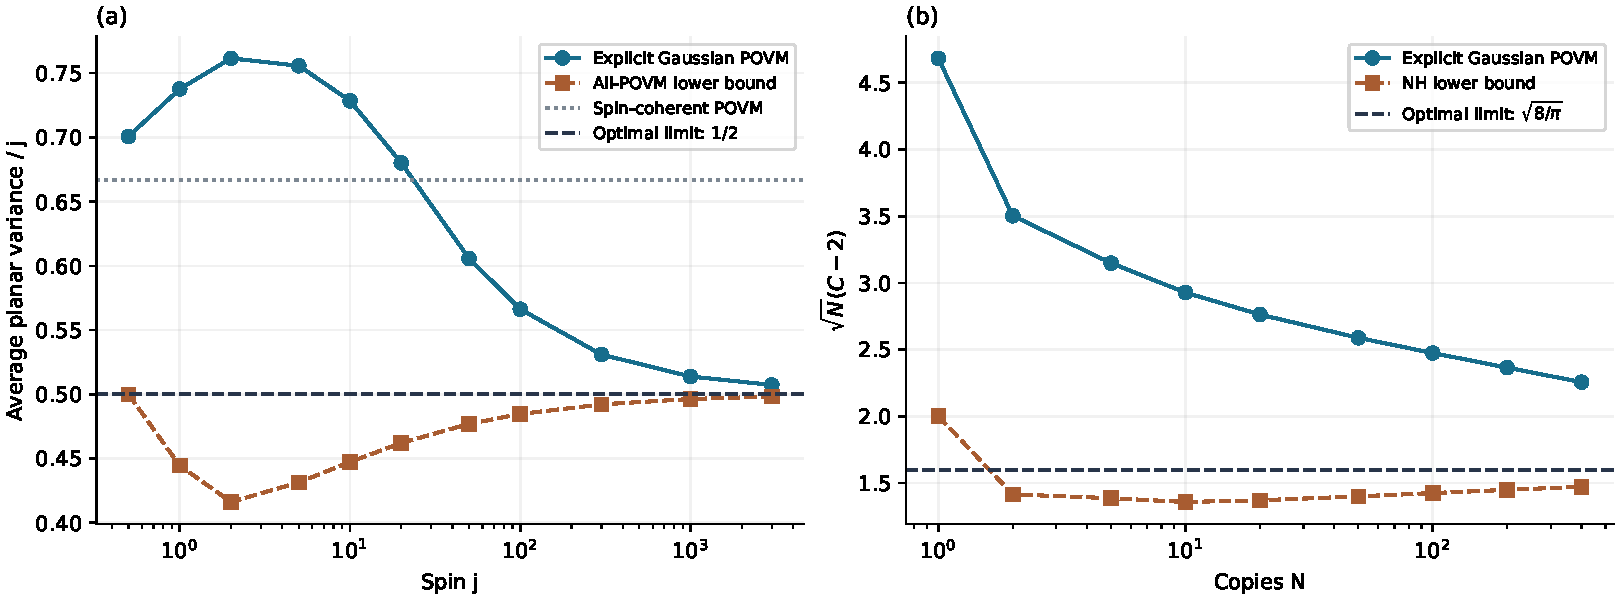
\includegraphics[width=\textwidth]{precision_scaling.pdf}
 \caption{\scalingcaption}
 \label{fig:scaling}
\end{figure*}

\section{讨论}\label{sec:discussion}

关键约束是测量种子的平均布居。局部压缩给出低方差态，
而合法测量还要求相应效应算子之和为恒等算子。
列归一化严格施加这一条件，同时保留调节宽度以控制方差的自由度。
赤道附近的正则化与两极处的估计，使局部压缩中的平衡可以贯穿整个自旋扇区。
这将已有的局部描述\cite{He2011,Dammeier2015}连接到可达的有限拷贝修正。

严格的 NH 间隙体现了有限规模下的同一完备性约束。
如附录~\ref{app:NH} 所示，在足够大的自旋扇区中，
饱和截顶证书的种子无法分解恒等算子。
高斯测量族严格满足完备性，而其方差与下界的差仅为 $o(j)$。
Schur 平均将这一差转化为 $o(\sqrt N)$ 的 Fisher 信息缺额，
以及归一化风险中 $o(N^{-1/2})$ 的间隙。
因此，NH 界在有限维下的不可达性与其首阶修正的准确性可以同时成立。

对数宽度序列给出了显式的渐近最优测量族，
而第~\ref{sec:gap}~节的有限 $N$ 例子表明，其收敛可能较慢。
针对有限拷贝表现优化宽度，以及确定更高阶修正，是自然的后续问题。
本文的结果针对最大混合态处的局部估计；若要将构造推广到非零参考 Bloch 向量，
则需处理扇区内状态及扇区概率的相应变化。

\section{结论}\label{sec:conclusions}

最大混合态处双参数量子比特估计的最优归一化风险为
$2+\sqrt{8/\pi}\,N^{-1/2}+o(N^{-1/2})$。
精确的高斯列分解达到相应的共同平均平面方差 $j/2+o(j)$，
其得分估计量对每个有限 $N$ 均严格局部无偏。
匹配的全 POVM 下界确定了首阶修正，并表明严格有限拷贝 NH 间隙属于更小的渐近阶。

\section*{数据与代码可用性}
[DATA AND CODE AVAILABILITY TO BE CONFIRMED]

\renewcommand{\acknowledgmentsname}{致谢}
\begin{acknowledgments}
[ACKNOWLEDGMENTS AND FUNDING TO BE COMPLETED]
\end{acknowledgments}

\section*{声明}
[DECLARATIONS TO BE CONFIRMED]

\appendix

\section{精确统计约化与种子表示}

\label{app:reduction}
本附录证明引理~\ref{lem:reduction}，并建立下界所用的种子表示。

\begin{proof}

整体参考态及切向算符分别为 $I/2^N$ 和 $2J_a^{\mathrm{tot}}/2^N$。
它们在分解 \eqref{eq:schur} 中为分块对角形式，在每个重数空间上均为标量。
对任意效应算子 $M_z$，定义
$E_{z|j}=\nu_j^{-1}\tr_{\mathrm{mult}}(\Pi_jM_z\Pi_j)$。
丢弃标签 $j$ 可恢复原测量的局部概率与导数；保留该标签则构成统计细化，
由 Cauchy--Schwarz 不等式，Fisher 信息在半正定序下增大。
反之，任意条件 POVM 都可提升为 $E_{z|j}\otimes I_{\nu_j}$。
由于 $\dot P_{N,j}=0$，其 Fisher 矩阵为条件矩阵的加权和。

对任意测量，令 $u(z)=\nabla\log p_\theta(z)|_0$，$F=\E_0[uu^{\mathsf T}]$。
若 $F$ 可逆，则估计量 $F^{-1}u$ 满足 \eqref{eq:unbiased}，协方差为 $F^{-1}$。
对每个局部无偏估计量，有
\[
 \E_0\bigl[(\widehat\theta-F^{-1}u)
 (\widehat\theta-F^{-1}u)^{\mathsf T}\bigr]
 =\Cov_0(\widehat\theta)-F^{-1}\succeq0.
\]
若 $F$ 奇异，恒等式 $\E_0[\widehat\theta u^{\mathsf T}]=I_2$ 不可能成立。
参考态满秩保证：以标量迹测度为控制测度时，这些得分恒等式也适用于连续测量结果。
特别地，得分有界。对正定 $F$，有 $\tr F^{-1}\geq4/\tr F$。
将测量绕 $z$ 轴随机旋转并保留旋转标签，可在不改变迹的前提下得到
$F=(\tr F/2)I_2$。这证明了前两个结论。

将效应算子细化至秩一不会减小 Fisher 信息。
$I/d$ 的纯态分解对应于效应算子 $E_a=dp_a\ket{\psi_a}\bra{\psi_a}$。
其概率为 $p_a$，得分为 $2(\ip{J_x}_{\psi_a},\ip{J_y}_{\psi_a})$。
完备性固定了
\[
 \sum_a p_a\ip{J_x^2+J_y^2}_{\psi_a}
 =\frac1d\tr(J_x^2+J_y^2)=\frac23j(j+1).
\]
减去平均方差即得到最后一个恒等式。

\end{proof}

为证明下界，先给出实非负种子形式。在以 $m=-j,\ldots,j$ 编号的 $J_z$ 基中，令
\begin{equation}
\begin{aligned}
c_m&=\sqrt{(j-m)(j+m+1)},\qquad
n_a=\sum_m v_{a,m}^2,\\
h_a&=\sum_{m=-j}^{j-1}c_mv_{a,m}v_{a,m+1}.
\end{aligned}
\label{eq:seeds}
\end{equation}
则
\begin{equation}
 T_j=\frac4d\max_{v_a\geq0,\;\sum_a v_{a,m}^2=1}
 \sum_a\frac{h_a^2}{n_a}.
 \label{eq:seed-opt}
\end{equation}
事实上，对复秩一向量 $w$，其对迹的贡献为 $4|\bra wJ_+\ket w|^2/(d\norm w^2)$。
将每个分量替换为其模，使该量不减并保持对角布居。
随后以如下相位轨道严格恢复完备性：
\begin{equation}
\begin{aligned}
E_{a\ell}&=\frac1L\ket{v_{a\ell}}\bra{v_{a\ell}},\qquad
v_{a\ell,m}=v_{a,m}e^{-im\phi_\ell},\\
\phi_\ell&=\frac{2\pi\ell}{L},\qquad L\geq\max(d,3).
\end{aligned}
\label{eq:phase-orbit}
\end{equation}
所有非零频率 $m-m'$ 的绝对值都小于 $L$，因而其相位平均为零。
一阶与二阶相位矩给出零均值得分及各向同性 Fisher 矩阵。
由于 $m-m'$ 总为整数，这一论证也适用于半整数自旋。

式 \eqref{eq:seed-opt} 中的最大值可以达到。为说明这一点，令
$p_{a,m}=v_{a,m}^2/n_a$，$\mu_a=n_a/d$。
它们在紧的概率单纯形上定义了均值为 $(1/d,\ldots,1/d)$ 的概率测度。
目标函数是连续函数 $4(\sum_mc_m\sqrt{p_mp_{m+1}})^2$ 的积分。
弱紧性保证最优解存在。在均匀向量处取其凹包络的支撑仿射函数，
再对接触集应用 Carath\'eodory 定理，可将支撑缩减为至多 $d$ 个种子。
我们仅在讨论严格的有限维间隙时使用最大值可达性。

\section{平方和下界}\label{sec:lower}

本附录证明定理~\ref{thm:main} 所用的全 POVM 下界，
并定义第~\ref{sec:gap}~节 NH 值中的截顶量。将 $d$ 个节点记为 $i=0,\ldots,d-1$，$d-1$ 条边记为 $i=0,\ldots,d-2$，
从而 $c_i=\sqrt{(i+1)(d-1-i)}$。对 $j>0$，令 $\tau_j$ 为下式的唯一正解：
\begin{equation}
 \sum_{i=0}^{d-2}(c_i-\tau_j)_+=\tau_j.
 \label{eq:cap}
\end{equation}
记
\begin{equation}
\begin{aligned}
a_i&=\min(c_i,\tau_j),\qquad S_j=\sum_i c_i a_i,\\
D_j&=\sum_i c_i^2-S_j,\qquad L_j=\frac{D_j}{d}.
\end{aligned}
\label{eq:cap-quantities}
\end{equation}
当 $j=0$ 时，以上四个量均取零。

\begin{proposition}\label{prop:lower}

对任意自旋均有 $V_j\geq L_j$。此外，
\begin{equation}
 L_j=\frac j2+o(j),\qquad 0\leq L_j\leq\frac j2+\frac14.
 \label{eq:lower-asymptotic}
\end{equation}
\end{proposition}

\begin{proof}

式 \eqref{eq:cap} 的左端减去右端所得函数连续且严格递减，
在零点为正，在 $\max_i c_i$ 处为负。定义
\[
 r_0=0,\qquad r_{i+1}-r_i=c_i/a_i-1.
\]
式 \eqref{eq:cap} 给出 $r_{d-1}=1$ 以及 $0\leq r_i\leq1$。
令 $a_{-1}=a_{d-1}=0$，并令
$\lambda_i=(1-r_{i-1})a_{i-1}^2+r_{i+1}a_i^2$，其中略去不存在的边界项。
若 $K$ 的非对角元为 $K_{i,i+1}=c_i$，则直接展开可得，对任意实向量 $v$ 和实数 $t$，
\begin{equation}
\begin{aligned}
&v^{\mathsf T}(\diag\lambda+t^2I-tK)v\\
&\quad=\sum_{i=0}^{d-1}\bigl[(1-r_i)(tv_i-a_iv_{i+1})^2\\
&\qquad\qquad{}+r_i(tv_i-a_{i-1}v_{i-1})^2\bigr]\geq0.
\end{aligned}
\label{eq:sos}
\end{equation}
这里，不存在的向量分量取零，并且 $a_i(1-r_i+r_{i+1})=c_i$。
此外，$\sum_i\lambda_i=S_j$。对非零种子，在式 \eqref{eq:sos} 中取 $t=h_a/n_a$，得到
$h_a^2/n_a\leq\sum_i\lambda_i v_{a,i}^2$。
对完备种子族求和可得 $T_j\leq4S_j/d$。
由于 $\sum_i c_i^2=\frac23j(j+1)d$，引理~\ref{lem:reduction} 给出 $V_j\geq D_j/d$。
因此，式 \eqref{eq:sos} 本身即为整个 POVM 优化问题的证书。

为证明渐近结论，令 $J=j+1/2=d/2$。此时
$c_i^2=J^2-(i+1-J)^2$ 且 $\tau_j<J$。截顶方程给出
\begin{equation}
 \tau_j^2\leq D_j=\sum_i c_i(c_i-\tau_j)_+
 \leq J\tau_j\leq J^2.
 \label{eq:cap-squeeze}
\end{equation}
假设存在 $\eta>0$，使得在某个无界子列上有 $\tau_j\leq(1-\eta)J$。
则中央固定正比例的边满足 $c_i\geq(1-\eta/2)J$，
它们对 $\sum_i(c_i-\tau_j)_+$ 的贡献为 $J^2$ 阶，与式 \eqref{eq:cap} 矛盾。
所以 $\tau_j/J\to1$，并且 $D_j/J^2\to1$。
将式 \eqref{eq:cap-squeeze} 除以 $d=2J$，即得两个结论。

\end{proof}

\section{高斯能量的全局估计}\label{sec:energy-proof}

本附录证明定理~\ref{thm:main} 所用的高斯方差上界。
式 \eqref{eq:W} 的分母将所有列耦合在一起；对 $h^2/s$ 使用下界，
可以将其转化为能够逐项一致估计的能量。令
\begin{equation}
\begin{aligned}
q(t)&=\sqrt{(J^2-t^2)_+},\qquad B_m=\sqrt{J^2-m^2},\\
k_m&=\frac{c_{m-1}+c_m}{2},
\end{aligned}
\label{eq:q}
\end{equation}
其中 $c_{-j-1}=c_j=0$。由 $h^2/s\geq2qh-q^2s$，有
\begin{equation}
\begin{aligned}
W_j[b]&\leq U_j[b]\\
&:=\frac1d\int_\R
\left[\sum_m(A_m+q^2)v_m^2-2qh_j\right]dt\\
&=\frac1d\left(\sum_m I_m+\sum_{m=-j}^{j-1}G_m+\sum_m R_m\right),
\end{aligned}
\label{eq:energy}
\end{equation}
其中各项均非负：
\begin{equation}
\begin{aligned}
I_m&=\int_\R(k_m-q(t))^2v_m(t)^2dt,\\
G_m&=c_m\int_\R q(t)(v_{m+1}(t)-v_m(t))^2dt,\\
R_m&=\frac{(c_m-c_{m-1})^2}{4}.
\end{aligned}
\label{eq:energies}
\end{equation}
式 \eqref{eq:energy} 中的第二个等号可由下式核实：
\begin{align*}
 h_j&=\sum_m k_mv_m^2-\frac12\sum_m c_m(v_{m+1}-v_m)^2,\\
 A_m-k_m^2&=R_m.
\end{align*}
\begin{theorem}\label{thm:energy}

对任意固定的正函数 $b\in C^2([-1,1])$，
\begin{equation}
 \lim_{j\to\infty}\frac{U_j[b]}j
 =\frac12\int_{-1}^1
 \left(x^2b(x)+\frac1{4b(x)}\right)dx.
 \label{eq:functional}
\end{equation}
取 $b_\epsilon(x)=(2\sqrt{x^2+\epsilon^2})^{-1}$ 及显式序列 \eqref{eq:epsilon}，则
\begin{equation}
 \frac{U_j[b_{\epsilon_j}]}j\longrightarrow\frac12,
 \qquad W_j[b_{\epsilon_j}]=\frac j2+o(j).
 \label{eq:explicit-energy}
\end{equation}
\end{theorem}

\subsection{两极处的一致控制}

本小节中所有记作 $C_b$ 的常数，仅依赖于 $b$ 的一个正下界及其 $C^2$ 范数的一个上界。
对 $r(s)=J-|s|\geq1/2$，有
\begin{equation}
\begin{aligned}
Jr(s)&\leq B(s)^2:=J^2-s^2\leq2Jr(s),\\
S(s)&\asymp_b r(s),\qquad |S'(s)|\leq C_b,\\
|S''(s)|&\leq C_b/J.
\end{aligned}
\label{eq:pole-scales}
\end{equation}
取正部的映射是 $1$-Lipschitz 的。因此，对每个实数 $t$，包括 $|t|\geq J$ 的情形，
\begin{equation}
 |q(t)-B_m|\leq\frac{|t^2-m^2|}{B_m}.
 \label{eq:global-q}
\end{equation}
在测度 $v_m(t)^2dt$ 下，$t-m$ 服从方差为 $S_m=S(m)$ 的正态分布。
由其二阶与四阶矩，得到
\begin{equation}
 \int(q-B_m)^2v_m^2dt
 \leq\frac{4m^2S_m+3S_m^2}{B_m^2}\leq C_bJ.
 \label{eq:position-bound}
\end{equation}
由于 $c_m=q(m+1/2)$，同一不等式还给出 $|k_m-B_m|^2\leq CJ/r(m)$。因此，对每一列均有
\begin{equation}
 0\leq I_m\leq C_bJ.
 \label{eq:I-bound}
\end{equation}
对梯度项，记 $Y=(t-s)/\sqrt{S(s)}$。直接求导得到
\begin{equation}
 \partial_sv_s=v_s\left[\frac{Y}{2\sqrt S}
 +\frac{S'}{4S}(Y^2-1)\right].
 \label{eq:derivative}
\end{equation}
平方根的 H\"older 不等式及式 \eqref{eq:pole-scales} 给出
\begin{align}
 q(s+\sqrt S Y)
 &\leq B(s)+\sqrt{2J\sqrt S|Y|+SY^2}\notag\\
 &\leq C_b\sqrt{Jr(s)}(1+|Y|).
 \label{eq:q-bound}
\end{align}
该界也包含所有越过两极的尾部。将高斯矩用于式 \eqref{eq:derivative}，得到
\begin{equation}
\begin{aligned}
&\int q(t)(\partial_sv_s(t))^2dt\\
&\quad\leq C_b\sqrt{Jr(s)}
\left(\frac1{S(s)}+\frac{S'(s)^2}{S(s)^2}\right)\\
&\quad\leq C_b\sqrt{\frac J{r(s)}}.
\end{aligned}
\label{eq:derivative-bound}
\end{equation}
当 $s\in[m,m+1]$ 时，$c_m\leq C\sqrt{Jr(s)}$。
因此，对 $s$ 使用积分形式的 Cauchy--Schwarz 不等式，有
\begin{equation}
\begin{aligned}
0\leq G_m
&\leq c_m\int_m^{m+1}\int q(t)(\partial_sv_s(t))^2dt\,ds\\
&\leq C_bJ.
\end{aligned}
\label{eq:G-bound}
\end{equation}
最后，$R_m\leq CJ/r(m)$，故
\begin{equation}
 \frac1d\sum_mR_m=O(\log(2+J))=o(J).
 \label{eq:R-bound}
\end{equation}
因此，对固定的 $0<\delta<1$，满足 $|m|>(1-\delta)J$ 的列及其关联边
对 $U_j[b]/J$ 的贡献至多为 $C_b(\delta+J^{-1})$。

\subsection{内部区域的极限}

固定 $\delta>0$，限制在满足 $|x_m|\leq1-\delta$ 的 $x_m=m/J$ 上。
以下误差在此集合上一致成立，常数可依赖于 $b$ 和 $\delta$。
令 $f(x)=\sqrt{1-x^2}$。中心展开给出 $k_m-B_m=O_\delta(J^{-1})$。
有如下全实轴余项估计：
\begin{equation}
\begin{aligned}
&\left|q(m+z)-B_m+\frac{m}{B_m}z\right|\\
&\quad\leq\left(\frac1{2B_m}+\frac{4m^2}{B_m^3}\right)z^2
             +\frac{z^4}{B_m^3}.
\end{aligned}
\label{eq:q-taylor}
\end{equation}
对任意实数 $u$ 和 $B>0$，有
$|\sqrt{u_+}-B-(u-B^2)/(2B)|\leq(u-B^2)^2/(2B^3)$；
取 $u=J^2-(m+z)^2$ 即得上述估计。因此，该式也覆盖 $q$ 为零的区域。
令 $z=\sqrt{Ja(x_m)}Y$，其右端为 $O_{b,\delta}(Y^2+J^{-1}Y^4)$。
平方后使用直至八阶的高斯矩，得到
\begin{equation}
\begin{aligned}
\frac{I_m}{J}
 &=a(x_m)f'(x_m)^2+O_{b,\delta}(J^{-1/2})\\
 &=x_m^2b(x_m)+O_{b,\delta}(J^{-1/2}).
\end{aligned}
\label{eq:I-limit}
\end{equation}
对梯度项，使用加权范数 $\norm w_q^2=\int q(t)|w(t)|^2dt$。
在内部的单位区间上，$S\asymp_{b,\delta}J$，$S'=O_b(1)$，$S''=O_b(J^{-1})$。
由式 \eqref{eq:derivative} 并再求一次导数，得到
\begin{equation}
\begin{aligned}
\norm{\partial_sv_s}_q&=O_{b,\delta}(1),\\
\norm{\partial_s^2v_s}_q&=O_{b,\delta}(J^{-1/2}).
\end{aligned}
\label{eq:H2}
\end{equation}
事实上，$\partial_s^2v_s/v_s$ 是关于 $Y$ 的至多四次多项式，
其系数为 $O_{b,\delta}(J^{-1})$，并且 $q\leq J$。
两次使用微积分基本定理，再使用 Minkowski 不等式，得到
\begin{equation}
\begin{aligned}
&\norm{v_{m+1}-v_m-\partial_mv_m}_q\\
&\quad\leq\int_m^{m+1}\int_m^s
\norm{\partial_u^2v_u}_qdu\,ds\\
&\quad=O_{b,\delta}(J^{-1/2}).
\end{aligned}
\label{eq:finite-diff}
\end{equation}
因此，$v_{m+1}-v_m$ 与 $\partial_mv_m$ 的范数平方相差 $O_{b,\delta}(J^{-1/2})$。
式 \eqref{eq:derivative} 中平移项的平方贡献为
\begin{align*}
 &\frac1{4Ja(x_m)}\E\bigl[q(m+\sqrt{Ja(x_m)}Y)Y^2\bigr]\\
 &\qquad=\frac{f(x_m)}{4a(x_m)}+O_{b,\delta}(J^{-1/2}).
\end{align*}
含 $S'$ 的交叉项为 $O_{b,\delta}(J^{-1/2})$，该项的平方为 $O_{b,\delta}(J^{-1})$。
由于 $c_m/J=f(x_m)+O_\delta(J^{-1})$，可得
\begin{equation}
 \frac{G_m}{J}=\frac1{4b(x_m)}+O_{b,\delta}(J^{-1/2}).
 \label{eq:G-limit}
\end{equation}
将式 \eqref{eq:I-limit} 和 \eqref{eq:G-limit} 中的 Riemann 和除以 $d=2J$，
得到式 \eqref{eq:functional} 在内部区域上的积分。
式 \eqref{eq:I-bound}、\eqref{eq:G-bound} 和 \eqref{eq:R-bound}
允许先令 $j\to\infty$，再令 $\delta\downarrow0$。
由于 $J/j\to1$，式 \eqref{eq:functional} 得证。

\subsection{一个显式宽度序列}

对式 \eqref{eq:functional} 的被积函数逐点极小化，提示在远离赤道处取 $b_*(x)=1/(2|x|)$。
我们使用如下正则化形式：
\begin{equation}
\begin{aligned}
b_\epsilon(x)&=\frac1{2\sqrt{x^2+\epsilon^2}},\\
a_\epsilon(x)&=\frac{1-x^2}{2\sqrt{x^2+\epsilon^2}},
\qquad 0<\epsilon\leq1.
\end{aligned}
\label{eq:regularized-width}
\end{equation}
精确积分给出极限泛函的值：
\begin{equation}
 \frac12\int_{-1}^1\left(x^2b_\epsilon+\frac1{4b_\epsilon}\right)dx
 =\frac12\sqrt{1+\epsilon^2}.
 \label{eq:integral}
\end{equation}
固定 $\epsilon$ 时，这已经推出 $\limsup_jV_j/j\leq\sqrt{1+\epsilon^2}/2$。
结合命题~\ref{prop:lower}，即证明式 \eqref{eq:roof-asymptotic}。
为了指定一个达到极限的测量族，我们保留上述估计对参数的依赖。

存在绝对常数 $C>0$，使得只要 $0<\delta<1/2$、$J\geq\epsilon^{-1}$
且 $J\delta\geq1$，便有
\begin{equation}
\begin{aligned}
&\left|\frac{U_j[b_\epsilon]}J-\frac12\sqrt{1+\epsilon^2}\right|\\
&\quad\leq C\epsilon^{-7}(\delta+J^{-1})\\
&\qquad{}+C(\epsilon^{-2}\delta^{-6}
             +\epsilon^{-12}\delta^{-4})J^{-1/2}
       +C\frac{1+\log(2J)}J.
\end{aligned}
\label{eq:uniform-error}
\end{equation}
下面给出支持这些指数的显式界。由式 \eqref{eq:regularized-width}，有
\begin{equation}
\begin{aligned}
\frac1{2\sqrt2}&\leq b_\epsilon\leq\frac1{2\epsilon},\\
\norm{a_\epsilon'}_\infty&\leq C\epsilon^{-3},\qquad
\norm{a_\epsilon''}_\infty\leq C\epsilon^{-5}.
\end{aligned}
\label{eq:parameter-bounds}
\end{equation}
于是，式 \eqref{eq:position-bound} 给出 $I_m\leq C\epsilon^{-2}J$。
式 \eqref{eq:q-bound} 中的常数可取为 $C\epsilon^{-1/2}$。
在式 \eqref{eq:derivative-bound} 中使用 $S\geq cr$ 及 $|S'|\leq C\epsilon^{-3}$，
得到 $G_m\leq C\epsilon^{-7}J$。
因此，分离出来的两极区域给出式 \eqref{eq:uniform-error} 的第一项；
对应的积分尾部至多为 $C\epsilon^{-1}\delta$。

在内部区域，$S\geq cJ\delta$，$S\leq CJ\epsilon^{-1}$，
且 $S',JS''$ 满足式 \eqref{eq:parameter-bounds} 中的多项式界。
为核对所有导数常数，将式 \eqref{eq:derivative} 的方括号写为
$g=A Y+B(Y^2-1)$，其中 $A=(2\sqrt S)^{-1}$，$B=S'/(4S)$。
则 $\partial_s^2v_s/v_s=g^2+\partial_sg$，且
\begin{align*}
 \partial_sY&=-S^{-1/2}-\frac{S'}{2S}Y,\qquad
 A'=-\frac{S'}{4S^{3/2}},\\
 B'&=\frac{S''}{4S}-\frac{S'^2}{4S^2}.
\end{align*}
$\partial_s^2v_s/v_s$ 中的四类系数为
$S^{-1}$、$S'/S^{3/2}$、$S''/S$ 和 $S'^2/S^2$。
因此，利用 $q\leq J$ 和固定阶高斯矩，得到
\begin{equation}
\begin{aligned}
\norm{\partial_sv_s}_q&\leq C\epsilon^{-3}\delta^{-1},\\
\norm{\partial_s^2v_s}_q&\leq C\epsilon^{-6}\delta^{-2}J^{-1/2}.
\end{aligned}
\label{eq:explicit-H2}
\end{equation}
因而，用导数替换有限差分所引起的范数平方变化至多为
$C\epsilon^{-12}\delta^{-4}J^{-1/2}$。
对位置项，使用全实轴余项式 \eqref{eq:q-taylor}、
$S\leq CJ\epsilon^{-1}$、$B_m\geq J\sqrt\delta$
以及 $|k_m-B_m|\leq CJ^{-1}\delta^{-3/2}$。
直至八阶的高斯矩给出一致界
\begin{equation}
 \left|I_m/J-x_m^2b_\epsilon(x_m)\right|
 \leq C\epsilon^{-2}\delta^{-6}J^{-1/2}.
 \label{eq:explicit-I}
\end{equation}
对梯度项的期望，可直接使用全局界 \eqref{eq:global-q}：
\begin{align*}
 &|q(m+\sqrt S Y)-B_m|\\
 &\quad\leq C\left[\sqrt J\epsilon^{-1/2}\delta^{-1/2}|Y|
             +\epsilon^{-1}\delta^{-1/2}Y^2\right].
\end{align*}
平移项平方、含 $S'$ 的交叉项以及含 $S'$ 项的平方所产生的误差，分别至多为
$C\epsilon^{-1}\delta^{-2}J^{-1/2}$、
$C\epsilon^{-3}\delta^{-2}J^{-1/2}$ 和 $C\epsilon^{-6}\delta^{-2}J^{-1}$。
计入式 \eqref{eq:explicit-H2} 以及将 $c_m/J$ 替换为 $f(x_m)$ 的变化，可得
\begin{equation}
 \left|G_m/J-1/(4b_\epsilon(x_m))\right|
 \leq C\epsilon^{-12}\delta^{-4}J^{-1/2}.
 \label{eq:explicit-G}
\end{equation}
最后，$x^2b_\epsilon+1/(4b_\epsilon)$ 的导数绝对值对所有 $\epsilon$
均不超过 $3/2$，从而控制了 Riemann 和的误差。这涵盖了前述论证的全部项，证明了式 \eqref{eq:uniform-error}。

现在采用式 \eqref{eq:epsilon}，并仅在证明中取 $\delta_j=\epsilon_j^8$。
两极误差为 $O(1/\log J)+O((\log J)^7/J)$，内部误差为
$O((\log J)^{50}/\sqrt J)$。
各项均趋于零，因此 $U_j[b_{\epsilon_j}]/j\to1/2$。
由 $L_j\leq V_j\leq W_j[b_{\epsilon_j}]\leq U_j[b_{\epsilon_j}]$，
式 \eqref{eq:explicit-energy} 成立。
截断参数 $\delta_j$ 不参与测量定义；所有列与全部实数结果 $t$ 均予以保留。

\section{Schur 平均与主定理证明的完成}\label{sec:averaging}

本附录对自旋界作 Schur 概率平均，完成定理~\ref{thm:main} 的证明。
记 $\E_N$ 为概率 $P_{N,j}$ 下的期望。下面的矩恒等式与余项估计控制了扇区数增长时的求和。

\begin{lemma}\label{lem:averaging}

Schur 概率满足
\begin{equation}
\begin{aligned}
\E_N[j(j+1)]&=\frac{3N}{4},\\
\frac{\E_Nj}{\sqrt N}&\longrightarrow\sqrt{\frac2\pi}.
\end{aligned}
\label{eq:schur-moments}
\end{equation}
设固定序列 $r_j$ 定义在所有非负整数与半整数自旋上，各项有限，且 $r_j=o(j)$，
则 $\E_Nr_j=o(\sqrt N)$。

\end{lemma}

\begin{proof}

第一个恒等式来自在态 $I/2^N$ 下对
$(J_x^{\mathrm{tot}})^2+(J_y^{\mathrm{tot}})^2+(J_z^{\mathrm{tot}})^2$ 求迹。
令 $S_N$ 为 $N$ 个独立对称符号变量之和。在
$P_{N,j}=(2j+1)(q_j-q_{j+1})$，
$q_j=2^{-N}\binom N{N/2-j}$ 中进行分部求和，得到精确恒等式
\begin{equation}
 \E_Nj=\E|S_N|-\frac12+\frac12\Pr(S_N=0).
 \label{eq:walk}
\end{equation}
相应的二项式和为
\[
 \E|S_{2n}|=2n\frac{\binom{2n}n}{2^{2n}},\qquad
 \E|S_{2n+1}|=(2n+1)\frac{\binom{2n}n}{2^{2n}}.
\]
由 Stirling 公式，式 \eqref{eq:schur-moments} 对奇偶两种情形均成立。
对任意 $\eta>0$，取固定的 $K_\eta$，使得 $j\geq K_\eta$ 时有 $|r_j|\leq\eta j$。
若 $M_\eta=\max_{j<K_\eta}|r_j|$，则
\[
 \frac{\E_N|r_j|}{\sqrt N}
 \leq\eta\frac{\E_Nj}{\sqrt N}+\frac{M_\eta}{\sqrt N}.
\]
先令 $N\to\infty$，再令 $\eta\downarrow0$，即得结论。
特别地，有限个小自旋值不影响这一结论。

\end{proof}

由定理~\ref{thm:energy} 和引理~\ref{lem:averaging}，
\begin{equation}
 \E_N W_j^{\g}=\frac12\sqrt{\frac2\pi}\sqrt N+o(\sqrt N).
 \label{eq:averaged-W}
\end{equation}
将 $W_j^{\g}$ 替换为 $V_j$ 或 $L_j$，同样的结论仍成立。对这三个序列中的任意一个 $Z_j$，
\begin{equation}
\begin{aligned}
\frac{4N}{2N-4\E_NZ_j}
 &=2+\frac{4\E_NZ_j}{N}+o(N^{-1/2})\\
 &=2+\sqrt{\frac8\pi}N^{-1/2}+o(N^{-1/2}).
\end{aligned}
\label{eq:risk-expansion}
\end{equation}
由命题~\ref{prop:lower}，下界适用于每个 POVM；显式测量族给出匹配的上界。
至此，定理~\ref{thm:main} 得证。

\section{NH 公式与严格有限拷贝分离}\label{app:NH}

本附录给出第~\ref{sec:gap}~节使用的有限维结论。
双参数 NH 界可表述为凸的一阶矩优化，等价地也可写为通常的半定松弛
\cite{HayashiOuyang2023,ZhangHayashi2026}。
令 $D=2^N$，对任意 Hermitian 一阶矩定义 $Z=X+iY$。
消去辅助算子块后，目标为
\[
\begin{aligned}
\mathcal F(Z)
 &=\min_{W\succeq Z^\dagger Z,\;W\succeq ZZ^\dagger}\tr W\\
 &=\tr Z^\dagger Z+
   \max_{0\preceq R\preceq I}\tr R(ZZ^\dagger-Z^\dagger Z).
\end{aligned}
\]
该等式可由 $ZZ^\dagger-Z^\dagger Z$ 的正谱部分得到。
归一化 NH 风险等于在一阶矩约束下将 $\mathcal F$ 最小化，再乘以 $N/D$。

在保留每个重数标签的 Schur 基底中，取对角矩阵 $R$，
其每个自旋块的对角元为附录~\ref{sec:lower} 中的 $r_i$。于是
\[
 \mathcal F(Z)\geq
 \sum_{\alpha,\beta}(1+r_\alpha-r_\beta)|Z_{\alpha\beta}|^2.
\]
所有系数均非负。在升算符边上，系数为
$1-r_i+r_{i+1}=c_i/a_i$。无偏条件给出
$\sum_{\text{raising edges}}c_i\operatorname{Re}Z_{i+1,i}=D$。
因此，在这些边上应用 Cauchy--Schwarz 不等式，得到
$\mathcal F(Z)\geq D^2/S_{\mathrm{tot}}$，其中
$S_{\mathrm{tot}}=\sum_j\nu_jS_j$。
该界对所有复矩阵 $Z$ 均成立，包括连接不同自旋块的矩阵元。

为达到此界，在每个扇区内取边元素 $x_{j,i}$ 为实非负数的相邻升算符矩阵，
并在重数空间上重复同一矩阵。设 $w_j=P_{N,j}/d$，其乘以 $N$ 之前的目标为
\begin{equation}
\begin{aligned}
&\sum_jw_j f_j(x_j),\\
f_j(x)&=\sum_i x_i^2+\frac12\sum_{i=0}^{d-1}|x_i^2-x_{i-1}^2|\\
&=\sum_{i=0}^{d-1}\max(x_{i-1}^2,x_i^2).
\end{aligned}
\label{eq:NH-objective}
\end{equation}
其中 $x_{-1}=x_{d-1}=0$。这些候选的均值与交叉导数均为零，
剩余的无偏性约束为 $\sum_jw_j\sum_i c_ix_{j,i}=1$。
以下包含 $S_j^{-1}$ 的表达式仅对 $j>0$ 的扇区求和；$j=0$ 扇区的贡献为零。
采用附录~\ref{sec:lower} 定义的 $r_i$，有
\begin{equation}
\begin{aligned}
f_j(x)&\geq\sum_i(1-r_i+r_{i+1})x_i^2\\
&=\sum_i\frac{c_i}{a_i}x_i^2
\geq\frac{(\sum_i c_ix_i)^2}{S_j}.
\end{aligned}
\label{eq:NH-CS}
\end{equation}
第一个不等式以两个分量的凸组合支撑各个最大值。
当 $x_i=a_i$ 时等号成立：$r_i$ 在每段未截顶的尾部选择较大的分量，
仅在平台区混合两个相等的分量。
第二个不等式为 Cauchy--Schwarz 不等式，在该取值下同样达到等号。
再对各扇区使用加权 Cauchy--Schwarz 不等式，证明最小值为 $1/\sum_jw_jS_j$，
并由 $x_{j,i}=a_{j,i}/\sum_kw_kS_k$ 达到。乘以 $N$，即得式 \eqref{eq:NH}。

现在假设式 \eqref{eq:seed-opt} 的种子最大值达到上界 $4S_j/d$。
于是每个种子在 $t=h/n\geq0$ 时均使式 \eqref{eq:sos} 的各非负项为零。
对 $t>0$，核空间的递推关系与连通性迫使非零种子的每个分量均为正。
若一条边满足 $c_i>\tau_j$，则 $r_{i+1}>0$ 且 $1-r_i>0$，
因此相邻两个方程迫使 $t=\tau_j$。
所有这样的种子均为同一个向量 $u$ 的倍数。
可将其平台区的分量设为一，并在左尾部得到
\begin{equation}
 u_i=(a_i/\tau_j)u_{i+1};
 \label{eq:tail-recursion}
\end{equation}
右尾部由反射得到。对 $t=0$，式 \eqref{eq:sos} 中的矩阵为对角矩阵，
仅有两个端点对应的对角元可能为零；内部所有 $\lambda_i$ 均严格为正。

若 $c_1<\tau_j$，则左侧前两条边均未截顶。
式 \eqref{eq:tail-recursion} 于是迫使每个正 $t$ 种子满足 $v_1=(c_1/\tau_j)v_2$，
而每个零 $t$ 种子在这两个节点均为零。
因此，各效应算子之和满足 $M_{11}=(c_1/\tau_j)^2M_{22}$，与 $M=I$ 不相容。
种子最大值的可达性使相应不等式严格成立。

为证明所有 $j\geq5$ 均满足 $c_1<\tau_j$，令 $n=2j\geq10$。
在 $n=10$ 时，中央六条边给出
\begin{align*}
 \sum_i(c_i-c_1)_+
 &=2(\sqrt{24}+\sqrt{28}+\sqrt{30})-6\sqrt{18}\\
 &>\sqrt{18}=c_1.
\end{align*}
可用纯有理数比较加以核对：这三个根式与 $\sqrt{18}$ 之比分别大于
$23/20$、$6/5$ 和 $5/4$，这些下界之和的两倍减六大于一。
对每个固定的 $i\geq2$，
\[
 \frac{c_i}{c_1}=
 \sqrt{\frac{(i+1)(n-i)}{2(n-1)}}
\]
随 $n$ 增大。三条边 $i=2,3,4$ 及其三条反射边，在 $n\geq10$ 时始终互不相同。
因此，对每个这样的 $n$ 都有 $\sum_i(c_i-c_1)_+>c_1$，
由式 \eqref{eq:cap} 的单调性可得 $\tau_j>c_1$。
当 $N\geq10$ 时，最大自旋扇区 $j=N/2$ 的概率为正，且具有严格的 Fisher 信息缺额，
从而 $C_N>C_N^{\nh}$。

% 由 REVTeX 自动选择 apsrev4-2，并保留文章题目控制项。
\bibliography{references}
\end{document}

